\documentclass{article}

\title{Dummit \& Foote Ch. 3.2: More on Cosets and Lagrange's Theorem}
\author{Scott Donaldson}
\date{Oct. 2023}
\usepackage{amsmath, amsthm, amsfonts, enumitem, tabu, tikz}

\begin{document}

\maketitle

Let $G$ be a group.

\section*{1. (10/1/23)}

Which of the following are permissible orders of subgroups of a group of order 120: 1, 2, 5, 7, 9, 15, 60, 240? For each permissible order give the corresponding index.

\begin{proof}
    From Lagrange's theorem, the order of a subgroup of a group of order 120 must divide 120. Then the permissible orders for subgroups are $1 = \frac{120}{120}$, $2 = \frac{120}{60}, 5 = \frac{120}{24}, 15 = \frac{120}{8}$, and $60 = \frac{120}{2}$. For each of these orders the index is given by the corresponding denumerator.
\end{proof}

\section*{2. (10/2/23)}

Prove that the lattice of subgroups of $S_3$ below is correct (i.e., prove that it contains all subgroups of $S_3$ and that their pairwise joins and intersections are correctly drawn).

\begin{center}
    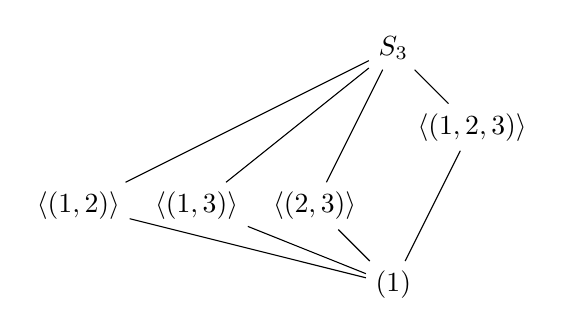
\begin{tikzpicture}
        \node at (0, 0)          (1)  {$(1)$};
        \node at (-4, 1)      (12)  {$\langle (1, 2) \rangle$};
        \node at (-2.5, 1)      (13) {$\langle (1, 3) \rangle$};
        \node at (-1, 1)      (23) {$\langle (2, 3) \rangle$};
        \node at (1, 2)      (123) {$\langle (1, 2, 3) \rangle$};
        \node at (0, 3)       (S3)  {$S_3$};
        
        \draw (1) -- (12);
        \draw (1) -- (13);
        \draw (1) -- (23);
        \draw (1) -- (123);
        \draw (12) -- (S3);
        \draw (13) -- (S3);
        \draw (23) -- (S3);
        \draw (123) -- (S3);
    \end{tikzpicture}
\end{center}

\begin{proof}
    The symmetric group $S_3$ contains 6 elements. By Lagrange's theorem, its proper subgroups must have order 2 or 3. Each of the subgroups in the lattice above have order 2 or 3, so there are no smaller or larger subgroups not depicted above.

    From Corollary 10, a subgroup of order 2 must be isomorphic to $Z_2$, that is, cyclic and generated by a single element of order 2. The three subgroups generated by the three elements of order 2 (the 2-cycles of $S_3$) are depicted above. Similarly, a subgroup of order 3 must be isomorphic to $Z_3$ and generated by a single element of order 3. The subgroup generated by $(1, 2, 3)$ contains $(1, 3, 2)$, so there is only a single subgroup of order 3.

    Next, again by Lagrange's Theorem, a subgroup of two different containing groups must have an order that divides the order of both of the containing groups. First consider a subgroup of order 2 and a subgroup of order 3. Only 1 divides 2 and 3, so the intersection must be the identity. Similarly, if a subgroup of order 2 and a subgroup of order 3 are contained in a larger group, then that group's order must have both 2 and 3 as divisors. The smallest integer for which this is possible is 6, which is the order of all of $S_3$.

    Finally, consider a pair of subgroups of order 2. Their intersection is either the identity or else they are the same subgroup. Their join must have even order, but 4 does not divide 6 and any larger even number exceeds the order of $S_3$. Thus their join is all of $S_3$. This concludes the proof that the lattice of subgroups of $S_3$ is correct.
\end{proof}

\section*{3. (10/2/23)}

Prove that the lattice of subgroups of $Q_8$ below is correct.

\begin{center}
    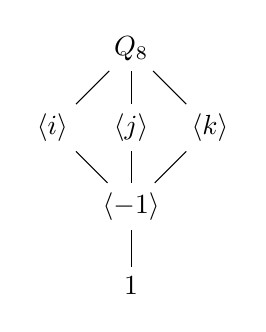
\begin{tikzpicture}
        \node at (0, 0)          (1)  {$1$};
        \node at (0, 1)      (-1)  {$\langle -1 \rangle$};
        \node at (-1, 2)      (i) {$\langle i \rangle$};
        \node at (0, 2)      (j) {$\langle j \rangle$};
        \node at (1, 2)      (k) {$\langle k \rangle$};
        \node at (0, 3)       (Q8)  {$Q_8$};
        
        \draw (1) -- (-1);
        \draw (-1) -- (i);
        \draw (-1) -- (j);
        \draw (-1) -- (k);
        \draw (i) -- (Q8);
        \draw (j) -- (Q8);
        \draw (k) -- (Q8);
    \end{tikzpicture}
\end{center}

\begin{proof}
    The group $Q_8$ has order $8 = 2^3$, so by Lagrange's theorem its proper subgroups must have order 2 or 4. We will start from the bottom and work toward the top: There is only one element of order 2 in $Q_8$, $-1$, and the cyclic subgroup generated by it is in the lattice.

    For each of $i, j$, and $k$, $\langle -1 \rangle$ is contained in the subgroup generated by them (ex. $\langle i \rangle = \{ \pm{1}, \pm{i} \}$) and there are no intermediate subgroups, since there is no divisor of 4 that is strictly greater than 2. At this point, every element of $Q_8$ is represented, so there are no cyclic subgroups missing. We might ask if there is a subgroup of order 4 missing. If so, it cannot be cyclic, and from Ch. 1.1, Exercise 36, it must be isomorphic to $V_4$. However, $V_4$ contains three elements of order 2, and $Q_8$ only has one, so there is no subgroup of $Q_8$ isomorphic to $V_4$.

    Finally, the join of any of the subgroups generated by $i, j$, or $k$ must contain strictly more than 4 elements and its order must divide 8. Then any of their joins must have order 8, that is, be all of $Q_8$.
\end{proof}

\section*{4. (10/3/23)}

Show that if $|G| = pq$ for some primes $p$ and $q$ (not necessarily distinct) then either $G$ is abelian or $Z(G) = 1$.

\begin{proof}
    We will show, equivalently, that if $|Z(G)| > 1$, then $G$ is abelian.
    
    Let $x \in Z(G)$. From Corollary 9, the order of $x$ divides $|G| = pq$. If $|x| = pq$, then $G = \langle x \rangle$ and so is abelian. Suppose without loss of generality that $|x| = p$. Now since the center of a group is a subgroup, we must have $\langle x \rangle \leq Z(G)$. If there exists a $y \in Z(G), y \notin \langle x \rangle$, then the order of $Z(G)$ exceeds $p$ and must divide $pq$, then it must be all of $G$ and hence $G$ is abelian. So suppose $Z(G) = \langle x \rangle$.
    
    The center of a group is normal in that group, so $G/Z(G)$ is well-defined. Since $|Z(G)| = p$, it has $q$ cosets in $G$; that is, the quotient group $G/Z(G)$ has prime order $q$ and is thus isomorphic to $Z_q$, hence cyclic. From Ch. 3.1, Exercise 36., $G$ is thus abelian.
\end{proof}

\section*{5. (10/4/23)}

Let $H$ be a subgroup of $G$ and fix some element $g \in G$.

\begin{enumerate}[label=(\alph*), itemsep=0em]
    \item Prove that $gHg^{-1}$ is a subgroup of $G$ of the same order as $H$.
          \begin{proof}
            By definition elements of $gHg^{-1}$ can be written in the form $ghg^{-1}$ for some $h \in H$, so let $gh_1g^{-1}, gh_2g^{-1} \in gHg^{-1}$. Then we have:
            \begin{equation*}
                (gh_1g^{-1})(gh_2g^{-1})^{-1} = gh_1g^{-1}gh_2^{-1}g_1 = gh_1h_2^{-1}g^{-1} \in gHg^{-1},
            \end{equation*}
            so $gHg^{-1}$ fulfills the subgroup criterion and is thus a subgroup of $G$.

            Next, let $\varphi_g: H \rightarrow gHg^{-1}$ be defined by $\varphi_g(h) = ghg^{-1}$ for all $h \in H$. This map is injective by the cancellation laws: $gh_1g^{-1} = gh_2g^{-1}$ implies that $h_1 = h_2$. It is also surjective: Let $x \in gHg^{-1}$. By definition $x = ghg^{-1}$ for some $h \in H$, so $\varphi_g(h) = x$. Therefore $\varphi_g$ is a bijection, and so $H$ and $gHg^{-1}$ have the same order.
          \end{proof}
    \item Deduce that if $n \in \mathbb{Z}^+$ and $H$ is the unique subgroup of $G$ of order $n$ then $H \unlhd G$.

          Suppose that $H$ is the unique subgroup of order $n$ in $G$. Then for all $g \in G$, we must have $gHg^{-1} = H$ (it cannot be any other subgroup, because $|gHg^{-1}| = |H| = n$ and there is no other subgroup of order $n$ in $G$). It follows that $H$ is normal in $G$.
\end{enumerate}

\section*{6. (10/4/23)}

Let $H \leq G$ and let $g \in G$. Prove that if the right coset of $Hg$ equals \emph{some} left coset of $H$ in $G$ then it equals the left coset $gH$ and $g$ must be in $N_G(H)$.

\begin{proof}
    Suppose $Hg = xH$ for some $x \in G$. Now $g \in Hg$, so we must also have $g \in xH$. Then $g = xh$ for some $h \in H$. It follows that $x = gh^{-1}$. So $Hg = xH = (gh^{-1})H = gH$, which in turns implies that $gHg^{-1} = H$. Therefore $g \in N_G(H)$.
\end{proof}

\section*{7. (10/5/23)}

Let $H \leq G$ and define a relation $\sim$ on $G$ by $a \sim b$ if and only if $b^{-1}a \in H$. Prove that $\sim$ is an equivalence relation and describe the equivalence class of each $a \in G$. Use this to prove Proposition 4.

\begin{proof}
    Let $a, b, c \in G$. We have $a \sim a$, because $a^{-1} a = 1 \in H$. If $a \sim b$, then we have $b^{-1}a \in H$. Now $b \sim a = a^{-1}b = (b^{-1}a)^{-1} \in H$, since $H$ is closed under inverses, so $a \sim b$ implies that $b \sim a$ (and the logic holds in reverse). Finally, if $a \sim b$ and $b \sim c$, then $b^{-1}a, c^{-1}b \in H$. Then their product, $c^{-1}bb^{-1}a = c^{-1}a$, is an element of $H$, which implies $a \sim c$. The relation $\sim$ is reflexive, symmetric, and transitive, therefore it is an equivalence relation.

    Let $a \in G$ and let $b$ lie in the left coset $aH$, so $b = ah$ for some $h \in H$. Then $b^{-1}a = (ah)^{-1}a = h^{-1}a^{-1}a = h^{-1} \in H$, so $a \sim b$. This implies that $aH$ is a subset of the equivalence class of $a$. And, if we have $a \sim b$, then $b^{-1}a \in H$, so $b^{-1}a = h$ for some $h \in H$. It follows that $b = ah^{-1} \in aH$, so the equivalence class of $a$ is a subset of $aH$. Since each is contained in the other, the equivalence class of $a$ under $\sim$ is the left coset $aH$.

    Now Proposition 4 states that:
    \begin{itemize}[itemsep=0em]
        \item The set of left cosets of $H$ in $G$ form a partition of $G$.
        \item For all $a, b \in G, aH = bH$ if and only if $b^{-1}a \in H$.
        \item In particular, $aH = bH$ if and only if $a$ and $b$ are representatives of the same coset.
    \end{itemize}
    Since the equivalence class of $a$ under $\sim$ is exactly the left coset $aH$ and equivalence classes partition a set, the left cosets of $H$ in $G$ partition $G$. The proof for the remaining items follows directly from the proof above that $a \sim b \iff b^{-1}a \in H \iff b \in aH$.
\end{proof}

\section*{8. (10/6/23)}

Prove that if $H$ and $K$ are finite subgroups of $G$ whose orders are relatively prime then $H \cap K = 1$.

\begin{proof}
    Let $H, K \leq G$ be finite subgroups whose orders are relatively prime. Let $x \in H \cap K$, so $x \in H$ and $x \in K$. From Corollary 9, the order of $x$ divides the orders of both $H$ and $K$. Since $|H|$ and $|K|$ are relatively prime, the order of $x$ must be 1, therefore $x = 1$. It follows that $H \cap K = 1$.
\end{proof}

\section*{9. (10/12/23)}

This exercise outlines a proof of Cauchy's Theorem due to James McKay (\emph{Another proof of Cauchy's group theorem}, Amer. Math. Monthly, 66(1959), p. 119). Let $G$ be a finite group and let $p$ be a prime dividing $|G|$. Let $\mathcal{S}$ denote the set of $p$-tuples of elements of $G$ the product of whose coordinates is 1:
\begin{equation*}
    \mathcal{S} = \{ (x_1, x_2, ..., x_p) \mid x_1 x_2 ... x_p = 1 \}.
\end{equation*}

\begin{enumerate}[label=(\alph*), itemsep=0em]
    \item Show that $\mathcal{S}$ has $|G|^{p - 1}$ elements, hence has order divisible by $p$.
          \begin{proof}
            Construct an element of $\mathcal{S}$ coordinate by coordinate. There are $|G|$ choices for the first element $x_1$. There are again $|G|$ choices for the second element $x_2$. We proceed similarly until the final element, which must satisfy the constraint that the product of all coordinates is 1. Therefore the final element must be equal to $(x_1 x_2 ... x_{p - 1})^{-1}$. We have freely chosen $p - 1$ coordinates from among $|G|$ possibilities; therefore $|\mathcal{S}| = |G|^{p - 1}$.
          \end{proof}
\end{enumerate}
Define the relation $\sim$ on $\mathcal{S}$ by letting $\alpha \sim \beta$ if $\beta$ is a cyclic permutation of $\alpha$.
\begin{enumerate}[label=(\alph*), itemsep=0em, start=2]
    \item Show that a cyclic permutation of $\mathcal{S}$ is again an element of $\mathcal{S}$.
          \begin{proof}
            Since $\alpha \sim \beta$ implies that $\beta$ is a cyclic permutation of $\alpha$, we have
            \begin{equation*}
                \alpha = (x_1, x_2, ..., x_p) \Rightarrow \beta = (x_{1 + n}, x_{2 + n}, ..., x_{p + n}),
            \end{equation*}
            where the subscripts of elements of $\beta$ are taken mod $p$ (although wrapping from 1 to $p$, rather than 0 to $p - 1$).

            The product of the coordinates of $\alpha$ is:
            \begin{align*}
                1 = \prod \alpha &= x_1 x_2 ... x_p \\
                &= (x_1 ... x_n)(x_{n + 1} ... x_p) \\
                &= (x_{n + 1} ... x_p)(x_1 ... x_n) \text{ (if $ab = 1$, then $ab = ba$)} \\
                &= (x_{1 + n} ... x_{p - n + n})(x_{(p - n + 1) + n} ... x_{p + n}) \\
                &= x_{1 + n} ... x_{p + n} = \prod \beta,
            \end{align*}
            and so the product of $\beta$'s coordinates is 1, making it an element of $\mathcal{S}$.
          \end{proof}
    \item Prove that $\sim$ is an equivalence relation on $\mathcal{S}$.
          \begin{proof}
            Let $\alpha, \beta, \gamma \in \mathcal{S}$. The relation $\sim$ is:
            \begin{itemize}[itemsep=0em]
                \item Reflexive: Let $\alpha = (x_1, x_2, ..., x_p)$. Then $x_i = x_{i + 0}$ for all coordinates $x_i$, so $\alpha$ is a cyclic permutation of itself, and therefore $\alpha \sim \alpha$.
                \item Symmetric: Let $\alpha \sim \beta$, $\alpha, \beta$ indexed by $x, y$ respectively. Since $\beta$ is a cyclic permutation of $\alpha$, we have $y_i = x_{i + n}$ for all $i \in \{ 1, ..., p \}$ for some $n \in \mathbb{Z}$. It follows that $x_i = y_{i + (p - n)}$ (subscripts mod $p$ wrapping from 1 to $p$), so $\alpha$ is also a cyclic permutation of $\beta$, and therefore $\beta \sim \alpha$.
                \item Transitive: Let $\alpha \sim \beta$ and $\beta \sim \gamma$, with $\alpha, \beta$ as above and $\gamma$ indexed by $z$. We have $y_i = x_{i + n}$ and $z_i = y_{i + k}$ for some $k, n \in \mathbb{Z}$. It follows that $z_i = x_{i + k + n}$, which implies that $\gamma$ is a cyclic permutation of $\alpha$, so $\alpha \sim \gamma$.
            \end{itemize}
            Therefore $\sim$ is an equivalence relation on $\mathcal{S}$.
          \end{proof}
    \item Prove that an equivalence class contains a single element if and only if it is of the form $(x, x, ..., x)$ with $x^p = 1$.
          \begin{proof}
            First, let $\alpha = (x, ..., x)$ and let $\alpha \sim \beta$. Then $\beta$ is a cyclic permutation of $\alpha$. Since $\alpha$ consists of a single, repeated coordinate value, we must have $\beta = (x, ..., x) = \alpha$. Therefore the equivalence class of $\alpha$ consists only of itself.

            Next, let $\alpha \in \mathcal{S}$ and suppose that the equivalence class of $\alpha$ under $\sim$ consists only of $\alpha$. Suppose $\alpha = (x_1, x_2, ..., x_p)$. Let $\beta$ be a cyclic permutation of $\alpha$ shifted by 1: $\beta = (x_2, x_3..., x_p, x_1)$. Now $\beta$ is in the equivalence class of $\alpha$, but we must have $\beta = \alpha$, so $x_{i + 1} = x_i$ for all $x_i$. It follows that $x_2 = x_1, x_3 = x_2 = x_1$, and so every value is equal to $x_1$. Then we have $\alpha = (x_1, ..., x_1)$, which is of the form $(x, ..., x)$, and by definition we must have $x^p = 1$.
          \end{proof}
    \item Prove that every equivalence class has order 1 or $p$ (this uses the fact that $p$ is a \emph{prime}). Deduce that $|G|^{p - 1} = k + pd$, where $k$ is the number of classes of size 1 and $d$ is the number of classes of size $p$.
          \begin{proof}
            From (d), if $\alpha = (x, ..., x)$ for some $x \in G$, its equivalence class has order 1.

            Let $\alpha = (x_1, x_2, ..., x_p)$. Then there are exactly $p$ members in the equivalence class of $\alpha$, and they are the cyclic permutations of $\alpha$ shifted by $0, 1, 2, ..., p - 1$, respectively. For example, the $n$-th member of the equivalence class is $(x_{1 + n}, x_{2 + n}, ..., x_{p + n})$.

            The equivalence classes of the elements of $\mathcal{S}$ partition $\mathcal{S}$. Suppose there are $k$ equivalence classes of order 1, and $d$ equivalence classes of order $p$. From (a), the order of $\mathcal{S}$ is $|G|^{p - 1}$. Then we have $|G|^{p - 1} = k + pd$.
          \end{proof}
    \item Since $\{ (1, 1, ..., 1) \}$ is an equivalence class of size 1, conclude from (e) that there must be a nonidentity element $x$ in $G$ with $x^p = 1$, i.e., $G$ contains an element of order $p$.
          \begin{proof}
            From (e), we have $|G|^{p - 1} = k + pd$ for some $k, d \geq 0$. From (a), $p$ divides the order of $\mathcal{S} = |G|^{p - 1}$, so we can write $ps = k + pd$ for some $s > 0$. Then $k = ps - pd = p(s - d)$, and so $p$ divides $k$. Because $p$ is prime, this implies that $k > 1$, so there are at least two elements whose equivalence classes have size 1. We already know that one is the identity; therefore there must be some element $\alpha \in \mathcal{S}, \alpha \neq (1, ..., 1)$ whose equivalence class under $\sim$ has size 1. From (d), $\alpha = (x, ..., x)$ for some $x \in G$, and we thus have $x^p = 1$, which implies that $|x| = p$.
          \end{proof}
\end{enumerate}

\section*{10. (11/2/23)}

Suppose $H$ and $K$ are subgroups of finite index in the (possibly infinite) group $G$ with $|G : H| = m$ and $|G : K| = n$. Prove that l.c.m.$(m, n) \leq |G : H \cap K| \leq mn$. Deduce that if $m$ and $n$ are relatively prime then $|G : H \cap K| = |G : H| \cdot |G : K|$.

\begin{proof}
    Let $g \in G$. Now $H \cap K$ is a subgroup of $G$, so the left cosets of it partition $G$. Consider the left coset:
    \begin{equation*}
        g(H \cap K) = \{ gx \mid x \in H \cap K \} = \{ gx \mid x \in H \} \cap \{ gx \mid x \in K \} = gH \cap gK. 
    \end{equation*}
    Since $|G:H| = m$, there are $m$ unique left cosets of $H$ in $G$, and similarly there are $n$ unique left cosets of $K$ in $G$. Then there are most $mn$ unique intersections of a left coset of $H$ with a left coset of $K$. It follows that there are at most $mn$ left cosets of $H \cap K$ in $G$, and so $|G : H \cap K| \leq mn$.

    Since we now know that $H \cap K$ has finite index in $G$, it must also have finite index in $H$ and $K$, respectively. Let $|H : H \cap K| = r$. Then there are $r$ unique cosets of $H \cap K$ in $H$ and $m$ cosets of $H$ in $G$. We have:
    \begin{align*}
        H &= \bigcup_{i = 1}^r h_i(H \cap K) \text{ for some $h_1, ..., h_r \in H,$ and} \\
        G &= \bigcup_{j = 1}^m g_j H \text{ for some $g_1, ..., g_m \in G$, therefore} \\
        G &= \bigcup_{j = 1}^m g_j \Bigl( \bigcup_{i = 1}^r h_i (H \cap K) \Bigr),
    \end{align*}
    a partition of $G$ into $mr$ unique cosets of $H \cap K$, so the index of $H$ in $G$ divides the index of $H \cap K$ in $G$. An identical proof shows the same is true for $K$. Since $m$ and $n$ divide $|G : H \cap K|$, it must be no less than the least common multiple of the two. Therefore l.c.m.$(m, n) \leq |G : H \cap K| \leq mn$.

    Note that if $m$ and $n$ are relatively prime, then their least common multiple is their product, in which case $|G : H \cap K| = |G : H| \cdot |G : K|$.
\end{proof}

\section*{11. (11/2/23)}

Let $H \leq K \leq G$. Prove that $|G:H| = |G:K| \cdot |K:H|$ (do not assume $G$ is finite).

\begin{proof}
    The proof in Exercise 10 above generalizes to this case. Since we can partition $G$ into $|G:K|$ cosets of $K$ and $K$ into $|K:H|$ cosets of $H$, there are $|G:K| \cdot |K:H|$ unique cosets of $H$ in $G$, and so $|G:H| = |G:K| \cdot |K:H|$.
\end{proof}

\section*{12. (10/16/23)}

Let $H \leq G$. Prove that the map $x \mapsto x^{-1}$ sends each left coset of $H$ in $G$ onto a right coset of $H$ and gives a bijection between the set of left cosets and the set of right cosets of $H$ in $G$ (hence the number of left cosets of $H$ in $G$ equals the number of right cosets).

\begin{proof}
    Let $\varphi: G \rightarrow G$ be defined by $\varphi(x) = x^{-1}$ for all $x \in G$. Consider:
    \begin{equation*}
        \varphi(xH) = \{ \varphi(xh) \mid h \in H \} = \{ (xh)^{-1} \mid h \in H \} = \{ h^{-1} x^{-1} \mid h \in H \} = Hx^{-1},
    \end{equation*}
    so $\varphi$ maps left cosets of $H$ onto right cosets of $H$.

    Further, considering $\varphi$ as a map from left cosets of $H$ to right cosets of $H$, it is a bijection.
    
    Toward injectivity, suppose that $\varphi(xH) = \varphi(yH)$ for some $x, y \in G$, and let $z \in xH$. Then $\varphi(z) = z^{-1} = hy^{-1}$, because $z \in xH$ and $\varphi(xH) = \varphi(yH)$. Inverting both sides, we obtain $z = (hy^{-1})^{-1} = yh^{-1} \in yH$, and so $xH \subseteq yH$. The same logic shows that $yH \subseteq xH$, so we must have $xH = yH$, and therefore $\varphi$ is injective.

    It is also surjective: Letting $Hx$ be a right coset of $H$, by definition we have $\varphi(x^{-1}H) = Hx$. It is therefore a bijection, and so there are an equal number of left cosets and right cosets of $H$ in $G$. 
\end{proof}

\section*{13. (10/16/23)}

Fix any labelling of the vertices of a square and use this to identify $D_8$ as a subgroup of $S_4$. Prove that the elements of $D_8$ and $\langle (1, 2, 3) \rangle$ do not commute in $S_4$.

\begin{proof}
    Label the vertices of a square starting at the upper-left corner and going clockwise 1, 2, 3, 4. We can assign to the generators $r, s$ of $D_8$ the permutations $(1, 2, 3, 4), (2, 4) \in S_4$, respectively.

    To show that the elements of $D_8$ and $\langle (1, 2, 3) \rangle$ do not commute, we note that:
    \begin{align*}
        (1, 2, 3) \cdot s &= (1, 2, 3)(2, 4) = (1, 2, 4, 3), \text{ and} \\
        s \cdot (1, 2, 3) &= (2, 4)(1, 2, 3) = (1, 4, 2, 3),
    \end{align*}
    so $s$ does not commute with $(1, 2, 3) \in S_4$. Therefore $D_8$ and $\langle (1, 2, 3) \rangle$ are not commuting subgroups of $S_4$.
\end{proof}

\section*{14. (10/17/23)}

Prove that $S_4$ does not have a normal subgroup of order 8 or a normal subgroup of order 3.

\begin{proof}
    From Corollary 10, a subgroup of order 3 is isomorphic to $Z_3$, hence cyclic. So, without loss of generality, consider $\langle (1, 2, 3) \rangle \leq S_4$. Consider the conjugate of $(1, 2, 3)$ by $(1, 2)(3, 4)$:
    \begin{equation*}
        (1, 2)(3, 4) \cdot (1, 2, 3) \cdot (1, 2)(3, 4) = (1, 4, 2),
    \end{equation*}
    which is not an element of $\langle (1, 2, 3) \rangle$. Therefore there is an element of $S_4$ that does not normalize $\langle (1, 2, 3) \rangle$ and, by isomorphism, any subgroup of order 3, so $S_4$ does not contain any normal subgroups of order 3.
    
    Next, let $X \leq S_4$ with $|X| = 8$ and suppose that $X \unlhd S_4$. From Cauchy's Theorem, $X$ contains an element of order 2, which may be either a single 2-cycle or a pair of disjoint 2-cycles. We will consider each case individually:
    \begin{itemize}
        \item Without loss of generality, suppose that $(1, 2) \in X$. Because $X$ is normal in $S_4$, the conjugate element $(1, 2, 3) \cdot (1, 2) \cdot (1, 3, 2) = (2, 3)$ must lie in $X$. Because $X$ is closed, the product $(1, 2) \cdot (2, 3) = (1, 2, 3)$ must lie in $X$, a contradiction since (from Corollary 9) a subgroup of order 8 contains no elements of order 3. Thus $X$ is not normal in $S_4$.
        \item Similarly, suppose that $(1, 2)(3, 4) \in X$. Again, the conjugate $(1, 2, 3) \cdot (1, 2)(3, 4) \cdot (1, 3, 2) = (1, 4, 3, 2)$ must lie in $X$. So the product $(1, 2)(3, 4) \cdot (1, 4, 3, 2) = (1, 3)$ must lie in $X$. Then, since $X$ contains a 2-cycle, it must contain an element of order 3, a contradiction. Thus $X$ is again not normal in $S_4$.
    \end{itemize}
    This concludes the proof that $S_4$ contains no normal subgroups of order 8 or order 3.
\end{proof}

\section*{15. (10/19/23)}

Let $G = S_n$ and for fixed $i \in \{ 1, 2, ...., n \}$ let $G_i$ be the stabilizer of $i$. Prove that $G \cong S_{n - 1}$.

\begin{proof}
    From Ch. 2.2, Exercise 8., we have defined a bijection $\varphi: G_i \rightarrow S_{n - 1}$ defined on a permutation $\sigma \in G_i$ and an element $m \in \{ 1, 2, ..., n \}$ it permutes:
    \begin{equation*}
        \varphi(\sigma)(m) =
        \begin{cases}
            \sigma(m)      & \text{if } \sigma(m) \leq i \\
            \sigma(m) - 1  & \text{if } \sigma(m) > i
        \end{cases}.
    \end{equation*}

    For $\sigma_1, \sigma_2 \in G_i$ and $m \in \{ 1, ..., n \}$, let $\sigma_2(m) = k$ and $\sigma_1(k) = p$. Let us consider the different cases for $k$ and $p$.
    
    \begin{enumerate}[itemsep=0em]
        \item $k \leq i, p \leq i$. Then:
              \begin{multline*}
                (\sigma_1 \circ \sigma_2)(m) = \sigma_1(\sigma_2(m)) = \sigma_1(k) = p \leq i, \text{ which implies that} \\
                \varphi(\sigma_1 \circ \sigma_2)(m) = (\sigma_1 \circ \sigma_2)(m) = p.
              \end{multline*}
              Also:
              \begin{align*}
                \sigma_2(m) = k \leq i \Rightarrow \varphi(\sigma_2(m)) = \sigma_2(m) = k, & \text{ and} \\
                \sigma_1(k) = p \leq i \Rightarrow \varphi(\sigma_1(k)) = \sigma_1(k) = p, & \text{ so} \\
                (\varphi(\sigma_1) \circ \varphi(\sigma_2))(m) &= \varphi(\sigma_1)\bigl(\varphi(\sigma_2)(m)\bigr) \\ &= \varphi(\sigma_1)\bigl(\sigma_2(m)\bigr) \\ &= \varphi(\sigma_1)(k) = \sigma_1(k) = p,
              \end{align*}
              thus $\varphi(\sigma_1 \circ \sigma_2) = \varphi(\sigma_1) \circ \varphi(\sigma_2)$.
        \item $k > i, p \leq i$. As above, we have $(\sigma_1 \circ \sigma_2)(m) = p \leq i$, which implies that $\varphi(\sigma_1 \circ \sigma_2)(m) = p$. Also:
              \begin{align*}
                \sigma_2(m) = k > i \Rightarrow \varphi(\sigma_2)(m) = \sigma_2(m) - 1 = k - 1.
              \end{align*}
              Now note that, in the permutation $\varphi(\sigma_1)$, all values greater than or equal to $i$ have been decremented by 1, so we have $\varphi(\sigma_1)(k - 1) = \sigma_1(k) = p$. It follows that:
              \begin{align*}
                (\varphi(\sigma_1) \circ \varphi(\sigma_2))(m) &= \varphi(\sigma_1)\bigl(\varphi(\sigma_2)(m)\bigr) \\ &= \varphi(\sigma_1)(k - 1) \\ &= \sigma_1(k) = p,
              \end{align*}
              thus $\varphi(\sigma_1 \circ \sigma_2) = \varphi(\sigma_1) \circ \varphi(\sigma_2)$.
        \item $k \leq i, p > i$. Then $(\sigma_1 \circ \sigma_2)(m) = p > i$, which implies that $\varphi(\sigma_1 \circ \sigma_2)(m) = (\sigma_1 \circ \sigma_2)(m) = p - 1$.
              As in the first case, $\varphi(\sigma_2)(m) = \sigma_2(m) = k$. So:
              \begin{align*}
                (\varphi(\sigma_1) \circ \varphi(\sigma_2))(m) &= \varphi(\sigma_1)\bigl(\varphi(\sigma_2)(m)\bigr) \\ &= \varphi(\sigma_1)(k) \\ &= \sigma_1(k) - 1 = p - 1,
              \end{align*}
              thus $\varphi(\sigma_1 \circ \sigma_2) = \varphi(\sigma_1) \circ \varphi(\sigma_2)$.
        \item $k > i, p > i$. As above, we have $\varphi(\sigma_1 \circ \sigma_2)(m) = p - 1$. As in the second case, we have $\varphi(\sigma_2)(m) = k - 1$; however, $\sigma_1(k) = p > i$, so $\varphi(\sigma_1(k - 1)) = \sigma_1(k) - 1 = p - 1$. Then:
              \begin{align*}
                (\varphi(\sigma_1) \circ \varphi(\sigma_2))(m) &= \varphi(\sigma_1)\bigl(\varphi(\sigma_2)(m)\bigr) \\ &= \varphi(\sigma_1)(k - 1) \\ &= \sigma_1(k - 1) - 1 = p - 1,
              \end{align*}
              thus $\varphi(\sigma_1 \circ \sigma_2) = \varphi(\sigma_1) \circ \varphi(\sigma_2)$.
    \end{enumerate}
    This exhaustively shows that for all $\sigma_1, \sigma_2 \in G_i$, the equation $\varphi(\sigma_1 \circ \sigma_2) = \varphi(\sigma_1) \circ \varphi(\sigma_2)$ holds in $S_{n - 1}$. Thus $\varphi$ is an isomorphism, and so $G_i \cong S_{n - 1}$.
\end{proof}

\section*{16. (10/19/23)}

Use Lagrange's Theorem in the multiplicative group $(\mathbb{Z}/p\mathbb{Z})^\times$ to prove \emph{Fermat's Little Theorem}: if $p$ is a prime then $a^p \equiv a \text{ (mod $p$)}$ for all $a \in \mathbb{Z}$.

\begin{proof}
    Recall that the order of the multiplicative group $(\mathbb{Z}/p\mathbb{Z})^\times$ is equal to the number of positive integers $n$ for which $n < p$ and $n$ is relatively prime to $p$. Since $p$ is prime, this is $p - 1$.

    For any $\overline{a} \in (\mathbb{Z}/p\mathbb{Z})^\times$, the order of $\overline{a}$ must divide $p - 1$, and in particular, we have $\overline{a}^{p - 1} = 1$. It follows that $\overline{a}^p = \overline{a}$. If $\overline{a} \in (\mathbb{Z}/p\mathbb{Z})^\times$ is a representative of some $a \in \mathbb{Z}$, we then conclude that $a^p \equiv a \text{ (mod $p$)}$.
\end{proof}

\section*{17. (10/19/23)}

Let $p$ be a prime and let $n$ be a positive integer. Find the order of $\overline{p}$ in \\ $(\mathbb{Z}/(p^n - 1)\mathbb{Z})^\times$ and deduce that $n \mid \varphi(p^n - 1)$ (here $\varphi$ is Euler's function).

\begin{proof}
    The order of $(\mathbb{Z}/(p^n - 1)\mathbb{Z})^\times$ is equal to the number of positive integers $k$ for which $k < p^n - 1$ and $k$ is relatively prime to $p^n - 1$, that is, $\varphi(p^n - 1)$.

    Now $p^n = (p^n - 1) + 1 \equiv 1 \text{ (mod $p^n - 1$)}$. For all non-negative $k < n$, we have $p^k < p^n$, so $n$ is the smallest positive integer for which $p^n \equiv 1 \text{ (mod $p^n - 1$)}$, which implies that $|\overline{p}| = n$. It follows that $n$ divides $\varphi(p^n - 1)$, the order of $(\mathbb{Z}/(p^n - 1)\mathbb{Z})^\times$.
\end{proof}

\section*{18. (11/3/23)}

Let $G$ be a finite group, let $H$ be a subgroup of $G$ and let $N \unlhd G$. Prove that if $|H|$ and $|G:N|$ are relatively prime then $H \leq N$.

\begin{proof}
    Toward contradiction, suppose that there exists an $h \in H, h \notin N$. The cyclic group $\langle hN \rangle$ is a subgroup of $G/N$, so its order divides $|G/N| = |G:N|$. Also, because for all $i, j \in \{ 0, ..., |h| - 1 \}$, $h^i N = h^j N$ implies $h^i = h^j$,$\langle hN \rangle$ has order equal to $|h|$, so $|h|$ divides $|G:N|$. Now since $|H|$ and $|G:N|$ are relatively prime and $|h|$ divides both, we must have $|h| = 1$, which implies that $h$ is the identity, and so lies in $N$, a contradiction.

    Therefore for all $h \in H$, we must have $h \in N$, and so $H \leq N$.
\end{proof}

\section*{19. (3/22/24)}

Prove that if $N$ is a normal subgroup of the finite group $G$ and $(|N|, |G:N|) = 1$ then $N$ is the unique subgroup of $G$ of order $|N|$.

\begin{proof}
    Suppose that $|N| = k$ and $|G| = mk$ with $k, m$ relatively prime. Let $A \leq G$ and suppose that $|A| = |N| = k$.

    Since $A \leq N_G(N) = G$, $AN$ is a subgroup of $G$. Then $|AN|$ must divide $mk$. Since $m$ and $k$ are relatively prime, $|AN|$ divides only one of either $m$ or $k$. Also, since $N \leq AN \leq G$, $|N| = k$ divides $|AN|$. We cannot have $k$ dividing $|AN|$ and $|AN|$ dividing $m$, therefore $|AN|$ both divides and is divided by $k$, so it must be equal to $k$.

    Now if there exists $a \in A$ such that $a \notin N$, then we would have $|AN| > k$. However, because $|AN| = k$, we must therefore have $A = N$. We conclude that $N$ is the unique subgroup of $G$ of order $k$.
\end{proof}

\section*{20. (3/21/24)}

If $A$ is an abelian group with $A \unlhd G$ and $B$ is any subgroup of $G$ prove that $A \cap B \unlhd AB$.

\begin{proof}
    Given $x \in A \cap B$, $g \in AB$, it suffices to show that $gxg^{-1} \in A \cap B$, or equivalenty that $gxg^{-1} \in A$ and $gxg^{-1} \in B$. Because $x \in A$ and $A \unlhd G$ (therefore $A \unlhd AB$) we already have $gxg^{-1} \in A$.

    To show that $gxg^{-1}$ also lies in $B$, from Corollary 15, we note that since $B \leq N_G(A) = G$, $AB$ is a subgroup of $G$. And from Corollary 14, since $AB$ is a subgroup, it follows that $AB = BA$. Write $g = ba$ for some $a \in A, b \in B$. Then:
    \begin{equation*}
        gxg^{-1} = (ba)x(ba)^{-1} = baxa^{-1}b^{-1} = \underbrace{baa^{-1}xb^{-1}}_{A \text{ is abelian and $x \in A$}} = \underbrace{bxb^{-1} \in B}_\text{$x \in B$},
    \end{equation*}
    and so $gxg^{-1} \in B$. Therefore $gxg^{-1} \in A \cap B$ for all $x \in A \cap B$, $g \in AB$, and so $A \cap B \unlhd AB$.
\end{proof}

\section*{21. (3/19/24)}

Prove that $\mathbb{Q}$ has no proper subgroups of finite index. Deduce that $\mathbb{Q}/\mathbb{Z}$ has no proper subgroups of finite index.

\begin{proof}
    We will first prove the more general case that a divisible abelian group has no proper subgroups of finite index, and then deduce that both $\mathbb{Q}$ and $\mathbb{Q}/\mathbb{Z}$ have no proper subgroups of finite index.

    Let $A$ be a divisible abelian group and let $B \leq A$. Since $A$ is abelian, all subgroups are normal, so the quotient group $A/B$ is well-defined. From Chapter 3.1, Exercise 15,  $A/B$ is also divisible. From Chapter 2.4, Exercise 19(b), no finite groups are divisible, so $|A:B| = |A/B| = \infty$.

    Since $\mathbb{Q}$ and $\mathbb{Q}/\mathbb{Z}$ are both divisible abelian groups, they therefore have no proper subgroups of finite index.
\end{proof}

\section*{22. (3/22/24)}

Use Lagrange's Theorem in the multiplicative group $(\mathbb{Z}/n\mathbb{Z})^\times$ to prove \emph{Euler's Theorem}: $a^{\varphi(n)} \equiv 1 \mod n$ for every integer $a$ relatively prime to $n$, where $\varphi$ denote's Euler's $\varphi$-function.

\begin{proof}
    Given $n \geq 2$, the order of $(\mathbb{Z}/n\mathbb{Z})^\times$ is $\varphi(n)$, the number of positive integers less than or equal to $n$ and relatively prime to $n$.

    Let $a \in \mathbb{Z}$ and consider $\overline{a} \in (\mathbb{Z}/n\mathbb{Z})^\times$. From Corollary 9, $\overline{a}^{|(\mathbb{Z}/n\mathbb{Z})^\times|} = \overline{a}^\varphi(n) = \overline{1}$. Therefore $a^{\varphi(n)} \equiv 1 \mod n$.
\end{proof}

\section*{23. (3/25/24)}

Determine the last two digits of $3^{3^{100}}$. [Determine $3^{100} \text{ mod } \varphi(100)$ and use the previous exercise.]

\begin{proof}[Solution]
    First, we note that $\varphi(100)$ — the number of integers relatively prime to and less than 100 — is 40 (this includes all and only numbers ending in 1, 3, 7, or 9). Next, note that $3^1 = 3, 3^2 = 9, 3^3 = 27, \text{ and } 3^4 = 81 \equiv 1 \text{ mod } 40$. It follows that $3^{100} = 3^{25 \cdot 4} \equiv 1 \text{ mod } 40$; that is, $3^{100} = 40n + 1$ for some $n \in \mathbb{Z}^+$.

    Now from the previous exercise, we know that $3^{\varphi(100)} = 3^{40} \equiv 1 \text{ mod } 100$. From above, we have $3^{100} \equiv 1 \text{ mod } 40$. Therefore:
    \begin{equation*}
        3^{3^{100}} = 3^{40n + 1} = 3^{40n} \cdot 3 \equiv (1 \cdot 3) \text{ mod } 100 = 3 \text{ mod } 100.
    \end{equation*}
    We conclude that $3^{3^{100}}$ ends in 03.
\end{proof}

\end{document}